\chapter{Potenciales termodinámicos}

\section{Transformadas de Legendre}

Las consecuencias físicas importantes del formalismo son más convenientes de ser exploradas al
considerar que la termodinámica puede ser reformulada en diversas formas teóricamente equivalentes.
Cada una de ellas es conveniente para algún tipo particular de problemas; la elección adecuada de la
formulación correcta simplifica considerablemente la resolución de los problemas. Por lo tanto, es
importante incorporar esto como un aspecto fundamental de la termodinámica.

De hecho, a lo largo del curso ya hemos considerado dos representaciones equivalentes, la
\textbf{representación entrópica} y la \textbf{representación energética}, aunque solo se ha
introducido formalmente un principio extremal, el \textbf{principio de máxima entropía}.

Para que ambas representaciones sean equivalentes, debe existir un principio análogo para dicha
representación. Tal principio existe; es equivalente y puede ser reemplazado por un
\textbf{principio de mínima energía}.

Notemos que el principio de máxima entropía caracteriza un estado de equilibrio como aquel que tiene
la máxima entropía para una energía total dada; el principio de mínima energía caracteriza el estado
de equilibrio como aquel que tiene la mínima energía para una entropía dada.

\subsection*{Equivalencia entre el principio de máxima entropía y el de mínima energía}

\begin{figure}[H]
  \centering
  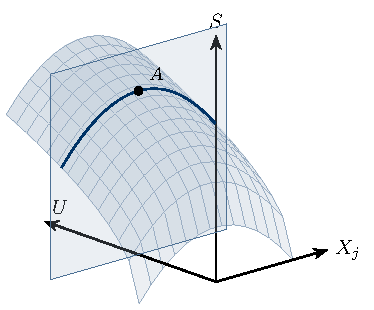
\includegraphics{figuras/plano-U0.pdf}
\end{figure}
La energía total del sistema es constante y determinada por la condición de cerradura ($U=U_0=\text{cte.}$);
geométricamente esta condición queda representada por el requerimiento de que los estados a los que
puede acceder el sistema se encuentran en el plano $U=U_0$. Asimismo, la relación fundamental se
representa por la hipersuperficie mostrada y el punto representativo del sistema debe estar en la
curva formada por la intersección del plano y la hipersuperficie. Si el parámetro $X_j$ no tiene
constricciones, el estado de equilibrio es el estado que \emph{maximiza} $S$ a lo largo de la curva
permitida; dicho estado es denotado por $A$.

La representación alternativa del estado de equilibrio $A$ como un estado de mínima energía para una
entropía dada es aquella donde el punto $A$ es alcanzado por el plano $S=S_0$, que determina una
curva dada por la intersección de dicho plano y la hipersuperficie dada por la relación
fundamental.
\begin{figure}[H]
  \centering
  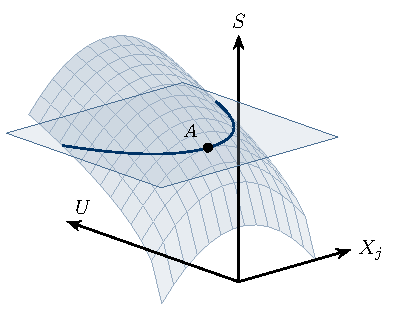
\includegraphics{figuras/plano-S0.pdf}
\end{figure}
Esta curva consiste de la familia de estados de entropía constante y el estado $A$ es el estado que
\emph{minimiza la energía} a lo largo de esta curva.
% NOTA: el manuscrito dice "es el estado que minimiza la entropía a lo largo de esta curva"; sobre la curva S=S_0 la entropía es constante, por lo que lo que se minimiza es la energía (así es en el principio de mínima energía que enuncia el propio manuscrito).

La equivalencia entre los principios de máxima entropía y de mínima energía depende del hecho de que
la forma geométrica de la hipersuperficie es en general de la forma mostrada en las figuras, la cual
está dada por los postulados $\pdv{S}{U}>0$ y que $U$ es una función continua y univaluada de $S$.
Aunque no se ha probado, se puede establecer la siguiente equivalencia:

\begin{postulado}[Principio de máxima entropía]
  El valor de equilibrio de cualquier parámetro interno no constreñido es tal que maximiza la
  entropía para un valor dado de la energía interna total.
\end{postulado}

\begin{proposicion}[Principio de mínima energía]
  El valor de equilibrio de cualquier parámetro interno no constreñido es tal que minimiza la
  energía para un valor dado de la entropía total.
\end{proposicion}
% NOTA: en el manuscrito el principio de mínima energía se enuncia como equivalente al de máxima entropía ("aunque no se ha probado"); aquí se rotula como proposición y se incluye la demostración que da el manuscrito (páginas siguientes), que muestra una implicación y deja la otra como "se demuestra de la misma forma".

\begin{proof}
Para demostrar el argumento de que ambos principios son equivalentes procedemos de la forma
siguiente. Asumamos el principio de máxima entropía: $\pdvc{S}{X}{U}=0$ implica que $S$ tiene un
extremo (con $X$ en lugar de $X_j$ por simplicidad), y asumamos también que
$\left(\dfrac{\partial^{2}S}{\partial X^{2}}\right)_{U}<0$, es decir, $S$ tiene un máximo.

Denotando también por simplicidad $P\equiv\pdvc{U}{X}{S}$ (aquí $P$ es el parámetro intensivo
conjugado de $X$) y de las relaciones implícitas que obtuvimos hace tiempo,
\begin{equation*}
  \pdvc{y}{x}{\psi,z}=-\frac{\pdvc{\psi}{x}{y,z}}{\pdvc{\psi}{y}{x,z}},
\end{equation*}
ya que queremos que $S$ aparezca,
\begin{equation*}
  P\equiv\pdvc{U}{X}{S}=-\frac{\pdvc{S}{X}{U}}{\pdvc{S}{U}{X}}=-\frac{\pdvc{S}{X}{U}}{1/T}=-T\pdvc{S}{X}{U},
\end{equation*}
donde se puede identificar $\pdvc{S}{U}{X}=\dfrac{1}{T}$. Por lo cual
\begin{equation*}
  P=-T\pdvc{S}{X}{U}=0.
\end{equation*}
Y por lo tanto $\pdvc{U}{X}{S}=0$ y $U$ es un extremo.

Para determinar qué tipo de extremo se tiene, se debe estudiar el signo de la segunda derivada
\begin{equation*}
  \left(\frac{\partial^{2}U}{\partial X^{2}}\right)_{S}\equiv\pdvc{P}{X}{S}.
\end{equation*}
Como $P=P(U,X)$ (no olvidar que no es la presión), por la regla de la cadena,
\begin{equation*}
  \left(\frac{\partial^{2}U}{\partial X^{2}}\right)_{S}=\pdvc{P}{X}{S}
  =\pdvc{P}{U}{X}\pdvc{U}{X}{S}+\pdvc{P}{X}{U}
  =\pdvc{P}{U}{X}P+\pdvc{P}{X}{U};
\end{equation*}
sin embargo, en el punto donde $U$ es un extremo, $P=\pdvc{U}{X}{S}=0$, por lo que
\begin{equation*}
  \left(\frac{\partial^{2}U}{\partial X^{2}}\right)_{S}=\pdvc{P}{X}{U}.
\end{equation*}
Aplicando de nuevo la derivada implícita, $P=-T\pdvc{S}{X}{U}$ con $T=\left(\pdvc{S}{U}{X}\right)^{-1}$,
\begin{equation*}
  \pdvc{P}{X}{U}=\pdv{X}\left[-\frac{\pdvc{S}{X}{U}}{\pdvc{S}{U}{X}}\right]_{U}
  =-\frac{\left(\partial^{2}S/\partial X^{2}\right)_{U}}{\pdvc{S}{U}{X}}
   +\pdvc{S}{X}{U}\,\frac{\partial^{2}S/\partial X\,\partial U}{\left(\pdvc{S}{U}{X}\right)^{2}}.
\end{equation*}
En el extremo $\pdvc{S}{X}{U}=0$, de modo que el segundo término se anula y
\begin{equation*}
  \boxed{\left(\frac{\partial^{2}U}{\partial X^{2}}\right)_{S}=-T\left(\frac{\partial^{2}S}{\partial X^{2}}\right)_{U}}
\end{equation*}
Como $\left(\dfrac{\partial^{2}S}{\partial X^{2}}\right)_{U}<0$ y $T>0$, se sigue que
$\left(\dfrac{\partial^{2}U}{\partial X^{2}}\right)_{S}>0$; por lo cual $U$ es un mínimo. El
argumento opuesto se demuestra de la misma forma y, por lo tanto, ambos principios son equivalentes.
\end{proof}

No se debe perder de vista que, independientemente del proceso seguido para alcanzar un estado de
equilibrio, en dicho estado se deben satisfacer ambos principios extremales.

Como ejemplo veamos la obtención de las condiciones de equilibrio térmico usando el principio de
mínima energía, en lugar del principio de máxima entropía. Consideremos un sistema cerrado compuesto,
con una pared rígida, impermeable y diatérmica. El calor es libre de fluir entre los dos subsistemas
y se busca encontrar el estado de equilibrio.
\begin{figure}[H]
  \centering
  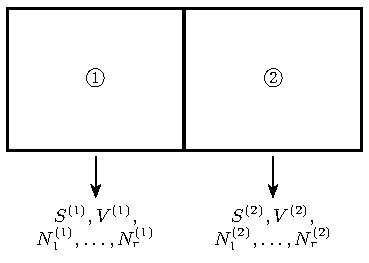
\includegraphics{figuras/cajas-entropia.pdf}
\end{figure}
La relación fundamental en la representación energética para el sistema compuesto es
\begin{equation*}
  U=U^{(1)}\bigl(S^{(1)},V^{(1)},N_1^{(1)},\dots\bigr)+U^{(2)}\bigl(S^{(2)},V^{(2)},N_1^{(2)},\dots\bigr).
\end{equation*}
En este caso se conocen los volúmenes (fijos) y los números de moles (fijos). Al permitir el flujo de
calor, solo $S^{(1)}$ y $S^{(2)}$ cambian.

Ahora, a pesar del hecho de que el sistema es cerrado y su energía total está fija, el estado de
equilibrio puede ser caracterizado como aquel que minimiza la energía si los cambios en la energía
son permitidos. El cambio en la energía total asociado con flujos de calor virtual entre los dos
subsistemas es
\begin{equation*}
  \dd U=T^{(1)}\,\dd S^{(1)}+T^{(2)}\,\dd S^{(2)}.
\end{equation*}
La condición de mínima energía establece que $\dd U=0$ y la condición de que la entropía total esté
fija establece que $S^{(1)}+S^{(2)}=\text{cte.}$; entonces
\begin{equation*}
  \dd U=0\quad\text{y}\quad\dd\bigl(S^{(1)}+S^{(2)}\bigr)=0;\qquad
  \dd S^{(1)}+\dd S^{(2)}=0\quad\text{o}\quad\dd S^{(1)}=-\dd S^{(2)},
\end{equation*}
\begin{equation*}
  \Longrightarrow\quad\dd U=0=T^{(1)}\,\dd S^{(1)}-T^{(2)}\,\dd S^{(1)}
  \quad\Longrightarrow\quad\dd U=\bigl[T^{(1)}-T^{(2)}\bigr]\,\dd S^{(1)}=0,
\end{equation*}
\begin{equation*}
  \boxed{T^{(1)}=T^{(2)}}
\end{equation*}
Por lo tanto, el principio de mínima energía produce el mismo resultado.

A través de $U=U^{(1)}+U^{(2)}$ y $T^{(1)}=T^{(2)}$ el problema está completamente resuelto. El resto de
condiciones de equilibrio puede ser encontrado de forma similar, aunque es más directo para la
energía que en el caso entrópico, donde se obtuvo $\dfrac{P^{(1)}}{T^{(1)}}=\dfrac{P^{(2)}}{T^{(2)}}$
(en la representación energética se obtiene directamente $P^{(1)}=P^{(2)}$).

\subsection*{Transformaciones de Legendre}

Para ambas representaciones (energética y entrópica) los parámetros extensivos juegan el rol de
variables independientes desde el punto de vista matemático. Esto contrasta con la situación que se
enfrenta experimentalmente, en la que usualmente es más fácil medir y controlar los parámetros
intensivos ($T$, $P$, \dots) que los parámetros extensivos (por ejemplo, no hay instrumentos para
medir la entropía, pero sí $T$; $S\leftrightarrow T$), lo que sugiere que es posible considerar a los
parámetros intensivos como las variables operacionalmente independientes y a los parámetros
extensivos como cantidades operacionalmente derivadas.

A los pares de variables termodinámicas entre parámetros extensivos e intensivos se les llama
\textbf{variables duales} o \textbf{conjugadas}. Estos son los pares de variables duales de un sistema
simple:
\begin{equation*}
  S\leftrightarrow T,\qquad V\leftrightarrow P,\qquad N\leftrightarrow\mu.
\end{equation*}
% NOTA: el manuscrito dice "entre parámetros extensivos y extensivos"; por el contexto (y los pares que se listan) es "extensivos e intensivos".

¿Es posible reconstruir el formalismo de la termodinámica de forma tal que los parámetros extensivos
sean reemplazados por los parámetros intensivos como variables matemáticas independientes?
% NOTA: el manuscrito dice "los parámetros extensivos sean reemplazados por los parámetros extensivos"; por el contexto es "por los parámetros intensivos".

Esto es posible y lleva a otras duales representaciones termodinámicas. La construcción de estas
representaciones es una cuestión de conveniencia, ya que la termodinámica tiene una estructura
lógica autocontenida en la representación entrópica o energética.

Para poder alcanzar este objetivo se recurre a las transformaciones de Legendre, las cuales permiten
cambiar una variable independiente en una función por otra que sea más conveniente.

\subsection*{Definición formal de la transformada de Legendre}

\begin{definicion}[Transformada de Legendre]
  Sea $f:\R^{n}\to\R$ una función convexa y diferenciable, $f=f(x_1,\dots,x_n)$, a valores reales. La
  \textbf{transformada de Legendre} de $f$ (aplicación que va de $\R^{n}$ a $\R$) es la función
  $f^{*}:\R^{n}\to\R$ definida como
  \begin{equation*}
    f^{*}(\vec{p})=\sup_{\vec{x}\in\R^{n}}\Bigl(\langle\vec{p},\vec{x}\rangle-f(\vec{x})\Bigr),
  \end{equation*}
  donde $\sup$ denota el supremo (el valor mayor posible), $\vec{x}$ es el vector $n$-dimensional de
  las variables independientes originales, $\vec{p}$ es el vector de las variables conjugadas,
  típicamente $\vec{p}=\nabla f(\vec{x})$, y $\langle\vec{p},\vec{x}\rangle$ es el producto interno
  entre $\vec{p}$ y $\vec{x}$.
\end{definicion}
% NOTA: en general f^{*}(p) solo es finita para los p en los que el supremo es finito (por ejemplo, para f(x)=e^x, f^{*}(p) solo está definida para p\geq0); la notación f^{*}:\R^{n}\to\R del manuscrito se usa aquí en el sentido usual de física, sobre el dominio en el que el supremo es alcanzado en un punto \vec{x} con \nabla f(\vec{x})=\vec{p}.

En $1$D esta relación puede simplificarse a
\begin{equation*}
  \boxed{f^{*}(p)=p\,x-f(x)\qquad\text{con }p=\frac{\dd f}{\dd x}}
\end{equation*}
Algunas de las consecuencias son que, si $f$ es estrictamente convexa y diferenciable, la
transformada de Legendre es \emph{involutiva}; es decir, al aplicar la transformada dos veces, se
recupera la función original.
% NOTA: la involución f^{**}=f requiere, en general, hipótesis adicionales (f convexa, semicontinua inferiormente y con \nabla f sobreyectiva sobre el dominio de f^{*}); vale, por ejemplo, para f de clase C^2 estrictamente convexa con f''>0 y crecimiento superlineal. Es el resultado usado en termodinámica.

Pasando al caso termodinámico, sea una relación fundamental de la forma
\begin{equation*}
  Y=Y(X_0,X_1,\dots,X_t)
\end{equation*}
con $X_i$ los parámetros extensivos del sistema. Por lo que se buscan
encontrar la forma de convertir a los parámetros intensivos $P_k\equiv\pdv{Y}{X_k}$ en variables
independientes \emph{sin perder contenido informacional} de $Y=Y(\vec{X})$ (de la relación
fundamental).

Dicho problema tiene su contraparte en geometría y en otras áreas de la física (por ejemplo, en
mecánica clásica) y se resuelve a través de las transformadas de Legendre. Su explicación es más clara
cuando se da una interpretación geométrica. Veamos el caso $1$D por simplicidad.

Sea una función (relación fundamental) que es función solo de una variable independiente $X$,
\begin{equation*}
  Y=Y(X).
\end{equation*}
Geométricamente, la relación fundamental se representa por una curva en un espacio con coordenadas
cartesianas $X$, $Y$.
\begin{figure}[H]
  \centering
  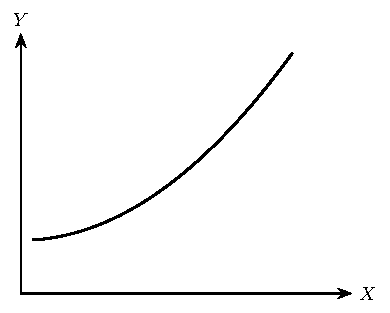
\includegraphics{figuras/curva-Y.pdf}
\end{figure}
Además, la derivada $P=\pdv{Y}{X}$ es la pendiente de dicha curva. Si solo se reemplaza $X$ por $P$,
para tener $Y=Y(P)$, \emph{inherentemente se pierde información}, ya que $\dd Y/\dd X$ no permite una
reconstrucción completa de la función $Y=Y(X)$. Debido a que $Y=Y(P)$ corresponde a diversas curvas de
igual pendiente, y desde el punto de vista analítico corresponde a una ecuación diferencial de primer
orden en $X$, solo puede ser calculada hasta una constante indeterminada.
\begin{figure}[H]
  \centering
  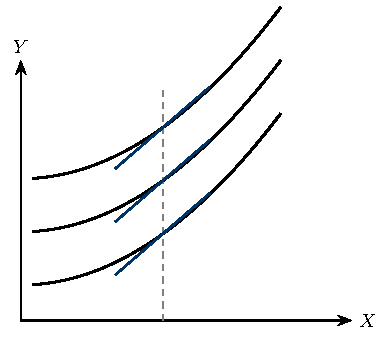
\includegraphics{figuras/familia-curvas.pdf}
\end{figure}

Este problema se resuelve a través de las transformadas de Legendre, las cuales son una consecuencia
de la dualidad (es decir, una relación fundamental) que existe en la geometría proyectiva y en la
teoría de líneas en los espacios tridimensionales, llamada \emph{dualidad entre la geometría de puntos
y la geometría de líneas de Plücker}.

\begin{observacion}[Digresión de topología]
  \textbf{Geometría proyectiva.} Rama de la geometría que estudia las propiedades de las figuras que
  son invariantes ante proyecciones. En la geometría euclidiana se preservan distancias y ángulos;
  en la proyectiva se preservan las relaciones de incidencia (qué puntos están en qué líneas) y las
  proporciones, en forma de razones dobles. Las transformaciones proyectivas son aquellas que se
  obtienen al proyectar una figura desde un punto sobre un plano y luego volver a proyectarla.

  \textbf{Geometría de líneas de Plücker} ($\mathbb{P}^{3}\subset\R^{4}$). En un espacio $3$D proyectivo,
  denotado por $\mathbb{P}^{3}$, que matemáticamente representa el conjunto de todas las rectas que
  pasan por el origen en un espacio $\R^{4}$, en lugar de puntos los objetos primarios son las líneas.
  $\mathbb{P}^{3}$ se representa por coordenadas homogéneas $[x_0:x_1:x_2:x_3]$, y
  $[\lambda x_0:\lambda x_1:\lambda x_2:\lambda x_3]$ representan al mismo punto para todo
  $\lambda\neq0$. Cada línea en $\mathbb{P}^{3}$ se representa con las coordenadas de Plücker
  $(p_{01},p_{02},p_{03},p_{12},p_{13},p_{23})$, que no son independientes, ya que deben satisfacer
  la ecuación de Plücker
  \begin{equation*}
    p_{01}p_{23}-p_{02}p_{13}+p_{03}p_{12}=0.
  \end{equation*}
  Esta ecuación define una variedad grassmanniana $G(1,3)$ (equivalentemente $\mathrm{Gr}(2,4)$) o
  variedad de líneas. Las $p$'s se definen a partir de dos puntos $P=[x_i]$ y $Q=[y_i]$ en
  $\mathbb{P}^{3}$ como $p_{ij}=x_iy_j-x_jy_i$ para $0\leq i<j\leq3$.
  % NOTA: el manuscrito rotula las coordenadas de Plücker como (p_12,p_13,p_14,p_23,p_24,p_34) y da la relación "p_12p_34+p_13p_24+p_14p_23=0", pero define p_ij para 0\leq i<j\leq3. Se unificó el índice (0 a 3, como en [x_0:x_1:x_2:x_3]) y se corrigió el signo del término central: la relación de Plücker correcta es p_01p_23 - p_02p_13 + p_03p_12 = 0 (por ejemplo, con x=(1,0,0,1), y=(0,1,1,0) se obtiene p_01=1, p_02=1, p_03=0, p_12=0, p_13=-1, p_23=-1, que la satisface solo con el signo menos).

  \textbf{Resumen.} Geometría proyectiva: propiedades de figuras invariantes ante proyecciones.
  Geometría de líneas: puntos $\to$ líneas ($\mathbb{P}^{3}\subset\R^{4}$, conjuntos de líneas,
  coordenadas de Plücker).
\end{observacion}

De forma resumida podemos decir que en la geometría proyectiva existe una correspondencia dual:
\begin{itemize}[itemsep=2pt]
  \item Un punto en el espacio proyectivo puede asociarse a un conjunto de líneas que pasan por este
    punto (un haz de líneas).
  \item Un plano puede asociarse a todas las líneas contenidas en él.
\end{itemize}
Por lo tanto, las coordenadas de Plücker permiten tratar a las líneas como puntos en un espacio
proyectivo de dimensión mayor ($\mathbb{P}^{5}$). Permite tratar problemas de intersección de líneas,
haces y congruencias de forma algebraica.

En nuestro caso, podemos decir lo siguiente. Una curva dada puede ser representada ya sea como:
\begin{enumerate}[label=\alph*),itemsep=0pt]
  \item la \emph{envolvente} de una familia de líneas tangentes (haz);
  \item el lugar geométrico de los puntos que cumplen la relación $Y=Y(X)$.
\end{enumerate}
\begin{figure}[H]
  \centering
  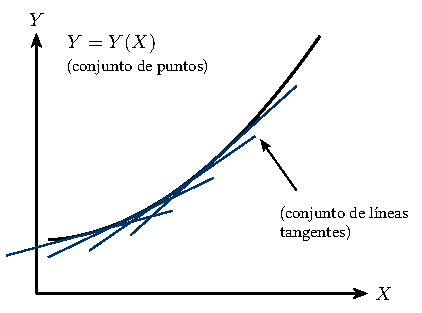
\includegraphics{figuras/tangentes.pdf}
\end{figure}
Por lo cual, cualquier ecuación que permita construir la familia de curvas tangentes también determina
la curva dada por $Y=Y(X)$.

Así como cada punto en el plano se determina por dos números $X$ y $Y$, cada línea recta en el plano
puede ser descrita por dos números $P$ y $\psi$, donde $P$ es la pendiente de la recta y $\psi$ la
ordenada al origen:
\begin{equation*}
  Y(X)=P\,X+\psi
\end{equation*}
Por lo que, debido a esta dualidad entre la geometría proyectiva y la geometría de Plücker, tal y como
una relación del tipo $Y=Y(X)$ selecciona un conjunto de todos los posibles pares ordenados $(X,Y)$
que cumplen con dicha relación, una relación del tipo $\psi=\psi(P)$ selecciona un subconjunto de
todas las líneas $(P,\psi)$.

Si se conocen las ordenadas al origen $\psi$ de las líneas tangentes en función de las pendientes $P$,
nos permite construir la familia de líneas tangentes y de ahí la curva de la cual estas líneas
tangentes son la envolvente. Por lo tanto, la relación $\psi=\psi(P)$ es completamente equivalente a
la relación fundamental $Y=Y(X)$. En la relación $\psi=\psi(P)$, $P$ es la variable independiente,
por lo que de esta forma se resuelve el problema planteado.

$\psi=\psi(P)$ es matemáticamente equivalente a la relación $Y=Y(X)$, y por lo tanto puede ser
considerada también una relación fundamental:
\begin{itemize}[itemsep=0pt]
  \item $Y=Y(X)$ es una relación fundamental en la ``representación $Y$'';
  \item $\psi=\psi(P)$ es la relación fundamental en la ``representación $\psi$''.
\end{itemize}

¿Cómo se puede calcular la relación $\psi=\psi(P)$ si se tiene la relación $Y=Y(X)$? Esto se puede
hacer a través de la transformada de Legendre; si se considera una línea tangente que pasa a través
del punto $(X,Y)$ y tiene pendiente $P$, y si la ordenada al origen es $\psi$, se tiene
\begin{figure}[H]
  \centering
  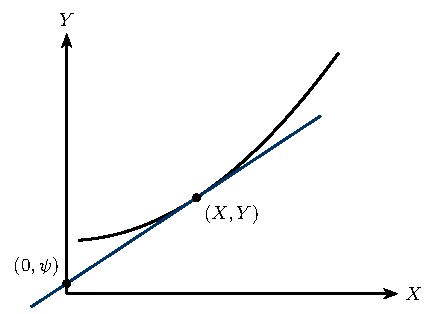
\includegraphics{figuras/tangente-psi.pdf}
\end{figure}
\begin{equation*}
  P=\frac{Y-\psi}{X-0}\quad\text{de acuerdo con el cálculo de la pendiente,}
  \qquad\text{o}\qquad
  \boxed{\psi=Y-PX}
\end{equation*}
% NOTA: con esta convención \psi(P)=Y-PX=-f^{*}(P), donde f^{*}(p)=px-f(x) es la transformada de la sección anterior; difieren solo en el signo.
Suponiendo que se tiene la ecuación $Y=Y(X)$, al diferenciar se obtiene
\begin{equation*}
  \frac{\dd Y}{\dd X}=P=P(X)
\end{equation*}
Al eliminar $X$ y $Y$ entre las ecuaciones
\begin{equation*}
  \psi=Y-PX,\qquad Y=Y(X),\qquad P=P(X),
\end{equation*}
se obtiene la relación buscada $\psi=\psi(P)$ (siempre que $P=P(X)$ sea invertible, es decir,
$\dd^{2}Y/\dd X^{2}\neq0$, para poder despejar $X=X(P)$). Como ya hemos visto, $\psi=Y-PX$ es la
definición analítica de la función $\psi$, y $\psi$ es llamada la \textbf{transformada de Legendre} de
$Y$.

El problema inverso es recuperar la relación $Y=Y(X)$ si la relación $\psi=\psi(P)$ es conocida. Para
encontrar la respuesta tomemos el diferencial de la transformada de Legendre,
\begin{equation*}
  \dd\psi=\dd Y-P\,\dd X-X\,\dd P,
\end{equation*}
pero recordando que $P=\dfrac{\dd Y}{\dd X}$, lo que implica que $\dd Y=P\,\dd X$, se tiene
\begin{equation*}
  \dd\psi=P\,\dd X-P\,\dd X-X\,\dd P=-X\,\dd P,
  \qquad\text{lo que implica que}\qquad
  \boxed{-X=\frac{\dd\psi}{\dd P}}
\end{equation*}
Y despejando la relación de la transformada de Legendre,
\begin{equation*}
  \boxed{Y=\psi+PX}
\end{equation*}
Si se eliminan las dos variables $\psi$ y $P$, se recupera entonces $Y=Y(X)$.

En resumen, la simetría entre las transformaciones de Legendre y su inversa se puede presentar como:
\begin{center}
  \renewcommand{\arraystretch}{1.3}
  \begin{tabular}{p{0.44\textwidth}|p{0.44\textwidth}}
    \textbf{Transformada de Legendre} & \textbf{Transformada inversa de Legendre}\\
    \hline
    $Y=Y(X)$ & $\psi=\psi(P)$\\
    $P=\dfrac{\dd Y}{\dd X}$ & $-X=\dfrac{\dd\psi}{\dd P}$\\
    $\psi=-PX+Y$ & $Y=XP+\psi$\\
    La eliminación de $X$ y $Y$ resulta en $\psi=\psi(P)$. & La eliminación de $P$ y $\psi$ resulta en $Y=Y(X)$.
  \end{tabular}
\end{center}

La generalización de esta transformada para más de $1$ variable independiente es directa. En $3$D,
$Y$ es una función de $X_0$ y $X_1$, y esta relación fundamental representa una superficie. Esta
superficie puede ser considerada como el lugar geométrico de los puntos que cumplen la ecuación
$Y=Y(X_0,X_1)$ o como la envolvente de los planos tangentes; asimismo, un plano puede ser
caracterizado por su ordenada al origen en el eje $Y$ y por las pendientes $P_0$ y $P_1$ de sus
trazas, en todos los posibles planos de un subconjunto descrito por $\psi=\psi(P_0,P_1)$.

En general, una relación fundamental
\begin{equation*}
  Y=Y(X_0,X_1,X_2,\dots,X_t)
\end{equation*}
representa una hipersuperficie en un espacio de dimensión $t+2$ con coordenadas cartesianas
$Y$, $X_0$, $X_1$, \dots, $X_t$. La derivada
\begin{equation*}
  P_k=\pdv{Y}{X_k}
\end{equation*}
es la pendiente parcial de dicha hipersuperficie.

Sea la relación fundamental $Y=Y(X_0,X_1,\dots,X_t)$, con $P_k=\pdv{Y}{X_k}$. La derivada parcial
denota la constancia de todas las variables naturales de $Y$, además de $X_k$ (es decir, de todas
las $X_j$ con $j\neq k$):
\begin{equation*}
  \dd Y=\sum_{k=0}^{t}P_k\,\dd X_k.
\end{equation*}
Se define la \textbf{transformada parcial de Legendre} (sobre las primeras $n+1$ variables) como
\begin{equation*}
  \boxed{Y[P_0,\dots,P_n]=Y-\sum_{k=0}^{n}P_kX_k}
\end{equation*}
La eliminación de $Y$ y $X_0,X_1,\dots,X_n$ de la relación fundamental y de las primeras $n+1$
ecuaciones nos da la transformada de la relación fundamental, $Y[P_0,\dots,P_n]$, función de
$P_0,P_1,\dots,P_n,X_{n+1},\dots,X_t$. Su diferencial es
\begin{equation*}
  \dd Y[P_0,\dots,P_n]=-\sum_{k=0}^{n}X_k\,\dd P_k+\sum_{k=n+1}^{t}P_k\,\dd X_k,
\end{equation*}
de modo que
\begin{align*}
  -X_k&=\pdv{Y[P_0,\dots,P_n]}{P_k}\qquad(k\leq n),\\
  P_k&=\pdv{Y[P_0,\dots,P_n]}{X_k}\qquad(k>n).
\end{align*}
La derivada parcial denota la constancia de todas las variables naturales de $Y[P_0,\dots,P_n]$
diferentes de aquellas sobre las que se lleva a cabo la diferenciación. La transformada inversa es
\begin{equation*}
  Y=Y[P_0,\dots,P_n]+\sum_{k=0}^{n}X_kP_k,
\end{equation*}
y al eliminar $Y[P_0,\dots,P_n]$ y $P_0,P_1,\dots,P_n$ de las ecuaciones anteriores y de las
primeras $n+1$ ecuaciones, nos lleva a la relación fundamental original.

\subsection*{Potenciales termodinámicos}

En el caso de la termodinámica, la aplicación de la transformada de Legendre es directa; en este
caso solo nos limitaremos al caso de las transformadas de Legendre que se derivan de la
representación energética $U=U(S,V,N_1,N_2,\dots)$ [las de la representación entrópica tienen sus
propias transformadas de Legendre, y son llamadas \emph{funciones de Massieu}], y las derivadas
$P_0,P_1,\dots$ corresponden a los parámetros intensivos $T,-P,\mu_1,\mu_2,\dots$

Estas transformadas de Legendre son llamadas \textbf{potenciales termodinámicos} y ahora veremos los
más comunes entre ellos. Cada uno de ellos tiene asociado un principio extremal y un significado
físico particular. Veamos cada uno de estos.

\subsubsection*{Energía libre de Helmholtz}

Es la transformada parcial de la energía interna $U$ que reemplaza a la entropía por la temperatura
como variable independiente. Usualmente se denota por $F$ o $A$. La relación fundamental en esta
representación es
\begin{equation*}
  F=F(T,V,N_1,N_2,\dots),
\end{equation*}
y en la notación usada es $F\equiv U[T]$. La energía libre de Helmholtz se puede sintetizar como
sigue. Se parte de la energía como relación fundamental, $U=U(S,V,N_1,N_2,\dots)$, donde
$T=\pdv{U}{S}$ es la temperatura. Entonces
\begin{equation*}
  \boxed{F=U-TS}
\end{equation*}
Al eliminar $U$ y $S$ en esta relación, se obtiene $F=F(T,V,N_1,N_2,\dots)$. Notemos que la
transformada inversa es
\begin{equation*}
  F=F(T,V,N_1,N_2,\dots)\quad\text{con}\quad-S=\pdv{F}{T}
  \;\Longrightarrow\;U=F+TS,
\end{equation*}
y al eliminar $F$ y $T$ se obtiene $U=U(S,V,N_1,N_2,\dots)$.

El diferencial completo de la energía libre de Helmholtz está dado por
\begin{equation*}
  \dd F=-S\,\dd T-P\,\dd V+\mu_1\,\dd N_1+\mu_2\,\dd N_2+\cdots
\end{equation*}
La energía libre de Helmholtz obedece el siguiente principio extremal.

\begin{ley}[Principio de mínima energía libre de Helmholtz]
  En un sistema cerrado, a volumen constante y a temperatura constante, el equilibrio se alcanza
  cuando la energía libre de Helmholtz es un mínimo:
  \begin{equation*}
    \pdvc{F}{X}{T,V,\dots}=0\qquad\text{y}\qquad\left(\frac{\partial^{2}F}{\partial X^{2}}\right)_{T,V,\dots}>0.
  \end{equation*}
\end{ley}
% NOTA: el manuscrito escribe "(\partial^2 F/\partial X^2)_{T,V}<0" junto a "es un mínimo"; para un mínimo la segunda derivada es positiva, por lo que se corrigió el signo. Ídem para la entalpía y la energía libre de Gibbs más adelante.

La interpretación física de la energía libre de Helmholtz es la siguiente: $F$ mide la capacidad de un
sistema para realizar trabajo útil (diferente a la expansión o contracción mecánica). Si $T$ y $V$ son
constantes:
\begin{enumerate}[label=\arabic*.,itemsep=0pt]
  \item El sistema intercambia energía con el entorno solo en forma de calor.
  \item Si $F$ decrece, se tiene que parte de la energía se convierte en trabajo útil.
\end{enumerate}

\subsubsection*{Entalpía}

Es la transformada parcial de Legendre de $U$ que reemplaza el volumen $V$ por la presión como
variable independiente. Usualmente se denota con el símbolo $H$. Las variables naturales de este
potencial son $S,P,N_1,N_2,\dots$ y se puede denotar como $H=U[P]$. Recordando que $-P=\pdv{U}{V}$, la
transformada de Legendre es
\begin{equation*}
  \boxed{H=U+PV}
\end{equation*}
y al eliminar $U$ y $V$ se tiene $H=H(S,P,N_1,N_2,\dots)$. Mientras que la transformada inversa de
Legendre parte de $H=H(S,P,N_1,N_2,\dots)$, con $V=\pdv{H}{P}$ y $U=H-PV$; al eliminar $H$ y $P$ se
obtiene $U=U(S,V,N_1,N_2,\dots)$. El diferencial total de la entalpía es
\begin{equation*}
  \dd H=T\,\dd S+V\,\dd P+\mu_1\,\dd N_1+\mu_2\,\dd N_2+\cdots
\end{equation*}

\begin{ley}[Principio de mínima entalpía]
  Para un sistema cerrado a $P$ y $S$ constantes, el equilibrio se alcanza cuando $H$ es un mínimo,
  es decir,
  \begin{equation*}
    \pdvc{H}{X}{S,P}=0\qquad\text{y}\qquad\left(\frac{\partial^{2}H}{\partial X^{2}}\right)_{S,P}>0.
  \end{equation*}
\end{ley}

$H$ representa la energía total del sistema más el trabajo de expansión ($PV$).
\begin{itemize}[itemsep=0pt]
  \item Si $P=\text{cte.}$ (en procesos abiertos a la atmósfera), la entalpía mide la energía
    disponible para cambios internos.
  \item La disminución de $H$ indica que el sistema libera energía (como calor) hasta alcanzar el
    estado más estable.
\end{itemize}

\subsubsection*{Energía libre de Gibbs}

El tercer potencial termodinámico común es la energía libre de Gibbs, la cual reemplaza
simultáneamente la entropía por la temperatura y al volumen por la presión. Este se denota
usualmente por $G$ y la relación fundamental tiene
variables naturales $T,P,N_1,N_2,\dots$ y se puede escribir $G\equiv U[T,P]$.

Sintetizando: de $U=U(S,V,N_1,N_2,\dots)$, con $T=\pdv{U}{S}$ y $-P=\pdv{U}{V}$, la transformada es
\begin{equation*}
  \boxed{G=U-TS+PV}
\end{equation*}
y al eliminar $U$, $S$ y $V$ se obtiene $G=G(T,P,N_1,N_2,\dots)$. Mientras que la transformada inversa
es $G=G(T,P,N_1,N_2,\dots)$, con
\begin{equation*}
  -S=\pdv{G}{T},\qquad V=\pdv{G}{P},\qquad U=G+TS-PV,
\end{equation*}
y al eliminar $G$, $T$ y $P$ resulta $U=U(S,V,N_1,N_2,\dots)$.

\begin{ley}[Principio de mínima energía libre de Gibbs]
  En un sistema cerrado a temperatura y presión constantes, el equilibrio se alcanza cuando la
  energía libre de Gibbs es un mínimo:
  \begin{equation*}
    \pdvc{G}{X}{T,P}=0\qquad\text{y}\qquad\left(\frac{\partial^{2}G}{\partial X^{2}}\right)_{T,P}>0.
  \end{equation*}
\end{ley}
% NOTA: el manuscrito escribe "(\partial^2 G/\partial X^2)_{T,P}<0" junto a "es un mínimo"; se corrigió el signo (ver la nota en la energía libre de Helmholtz).

$G$ mide la energía para realizar trabajo útil no volumétrico (eléctrico, químico, etc.) cuando $T$ y
$P$ son fijas. Cuando el sistema está en contacto con un termostato (baño térmico o $T$ fija) y con un
barostato (a condiciones de presión fija o reservorio de presión), cualquier cambio espontáneo reduce
$G$.

\section{Relaciones de Maxwell}

% Pendiente: aún no está en las notas.

\section{Estabilidad de sistemas termodinámicos}

% Pendiente: aún no está en las notas.

